\documentclass{beamer}

\mode<presentation> {
%\usetheme{default}
% \usetheme{AnnArbor}
%\usetheme{Antibes}
%\usetheme{Bergen}
%\usetheme{Berkeley}
\usetheme{Berlin}
%\usetheme{Boadilla}
%\usetheme{CambridgeUS}
%\usetheme{Copenhagen}
%\usetheme{Darmstadt}
%\usetheme{Dresden}
%\usetheme{Frankfurt}
%\usetheme{Goettingen}
%\usetheme{Hannover}
%\usetheme{Ilmenau}
%\usetheme{JuanLesPins}
%\usetheme{Luebeck}
% \usetheme{Madrid}
%\usetheme{Malmoe}
%\usetheme{Marburg}
%\usetheme{Montpellier}
%\usetheme{PaloAlto}
%\usetheme{Pittsburgh}
%\usetheme{Rochester}
%\usetheme{Singapore}
%\usetheme{Szeged}
% \usetheme{Warsaw}

%\usecolortheme{albatross}
\usecolortheme{beaver}
%\usecolortheme{beetle}
%\usecolortheme{crane}
%\usecolortheme{dolphin}
%\usecolortheme{dove}
%\usecolortheme{fly}
%\usecolortheme{lily}
%\usecolortheme{orchid}
%\usecolortheme{rose}
%\usecolortheme{seagull}
%\usecolortheme{seahorse}
%\usecolortheme{whale}
%\usecolortheme{wolverine}

\setbeamertemplate{footline} % To remove the footer line in all slides
%\setbeamertemplate{footline}[page number] % To replace the footer line in all slides
%\setbeamertemplate{navigation symbols}{} % remove the navigation symbols from the bottom of slides
}

\usepackage{graphicx}
\usepackage{booktabs}
\usepackage{bm}
\usepackage[lined,boxed]{algorithm2e}
\usepackage{hyperref}
\usepackage{pifont}


\newcommand{\iter}[2]{#1^{(#2)}}
\DeclareMathOperator*{\argmin}{arg\,min}
\DeclareMathOperator*{\argmax}{arg\,max}


%====================================================================================
%=======================================================================   TITLE PAGE
%====================================================================================
\title[Online MM]{Online MM Algorithms for Machine Learning}
\author{Josh Day}
\institute[NC State University]{NC State University \\ \textit{jtday2@ncsu.edu}}
\date{December 21, 2016}

\begin{document}

\begin{frame}
\titlepage
\end{frame}

% \begin{frame}
% \frametitle{Overview}
% \tableofcontents
% \end{frame}

%%%%%%%%%%%%%%%%%%%%%%%%%%%%%%%%%%%%%%%%%%%%%%%%%%%%%%%%%%%%%%%%%%%%%%%%%%%%%%%%%%%%% Intro
\section{Introduction}
%------------------------------------------------ Motivation
\subsection{Motivation}
\begin{frame}
  \begin{figure}
    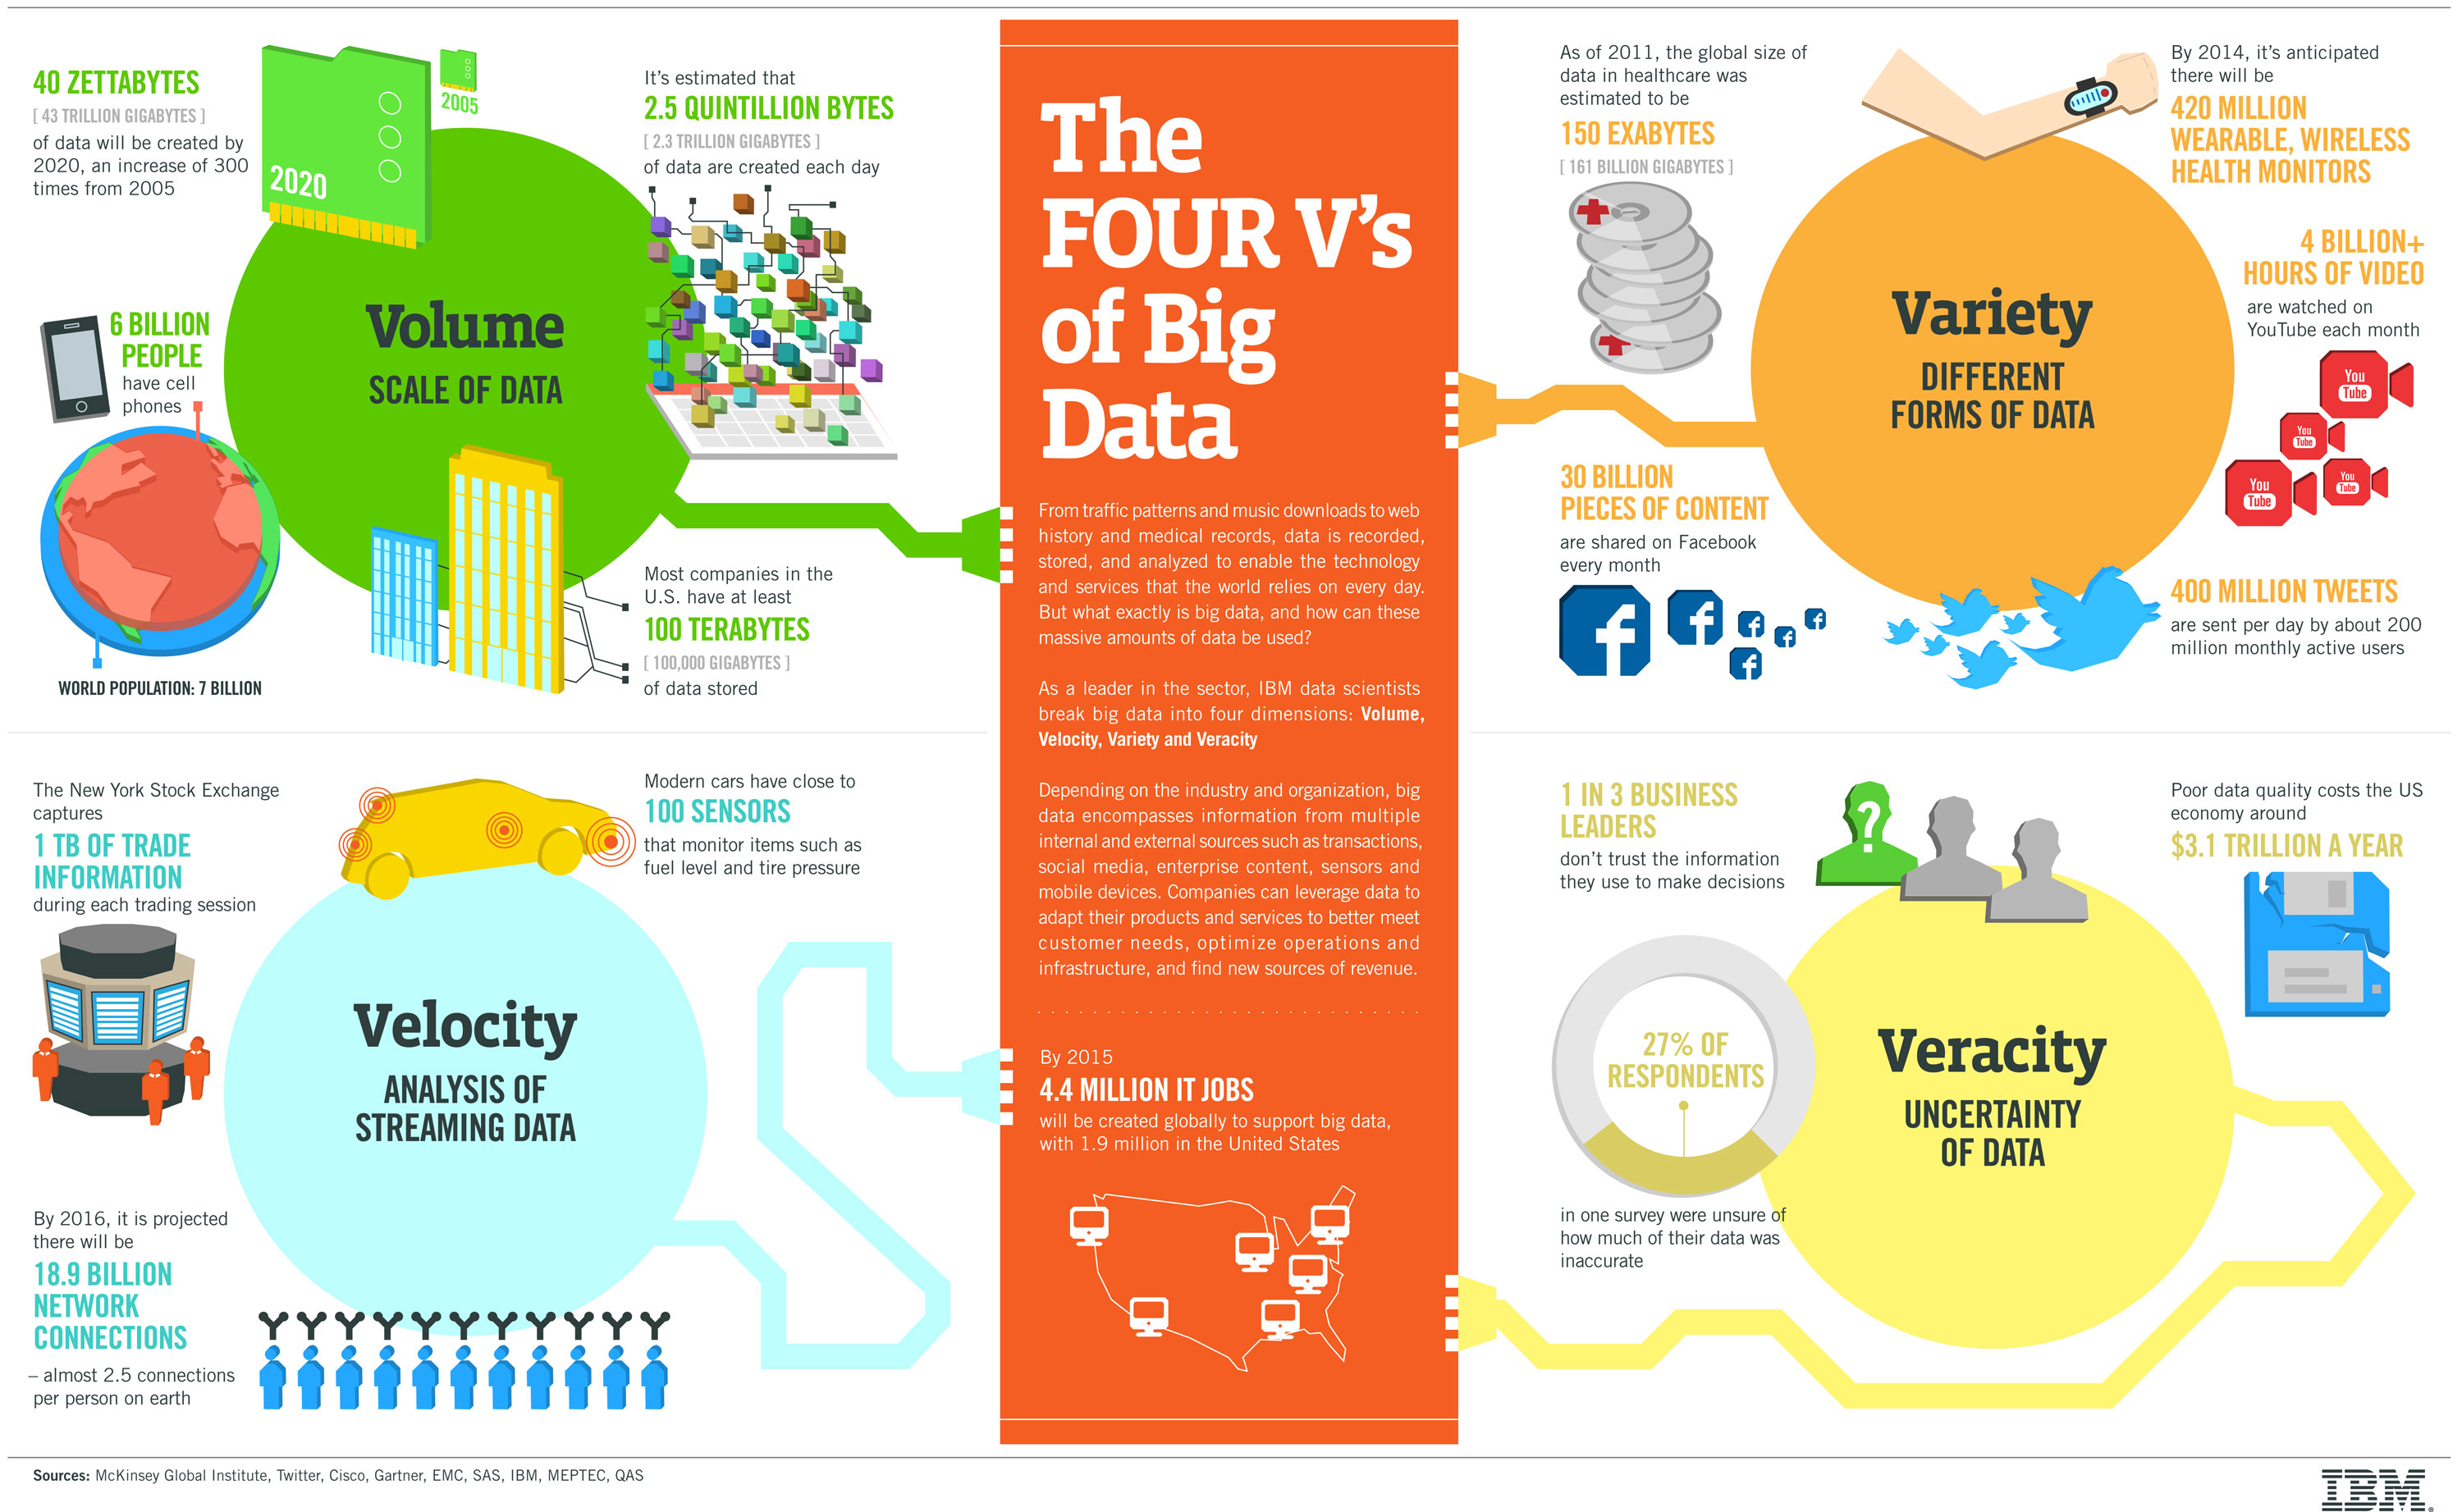
\includegraphics[width=\linewidth]{figures/4vs.jpg}
  \end{figure}
\end{frame}
\begin{frame}
  \begin{itemize}
    \item Statisticians don't have the tools to handle all of this
    \item Adapting our favorite algorithms is often nontrivial
    \item Note: If we can handle Velocity, we can handle Volume
  \end{itemize}
\end{frame}

%------------------------------------------------ What is MM
\subsection{MM Algorithms}
\begin{frame}
  \frametitle{What is a Majorization Minimization Algorithm?}
  \begin{itemize}
    \item $h$ is said to \emph{majorize}  $f$ at $\iter{\bm\theta}{t}$ if:
    $$\begin{aligned}
      h(\bm\theta|\iter{\bm\theta}{t}) &\ge f(\bm\theta|\iter{\bm\theta}{t}) \\
      h(\iter{\bm\theta}{t}|\iter{\bm\theta}{t}) &= f(\iter{\bm\theta}{t}|\iter{\bm\theta}{t})
    \end{aligned}$$
    \item MM update: $\bm\theta^{(t+1)} = \argmin_{\bm\theta} \; h(\bm\theta|\bm\theta^{(t)})$
  \end{itemize}
\end{frame}
\begin{frame}
  \begin{figure}
    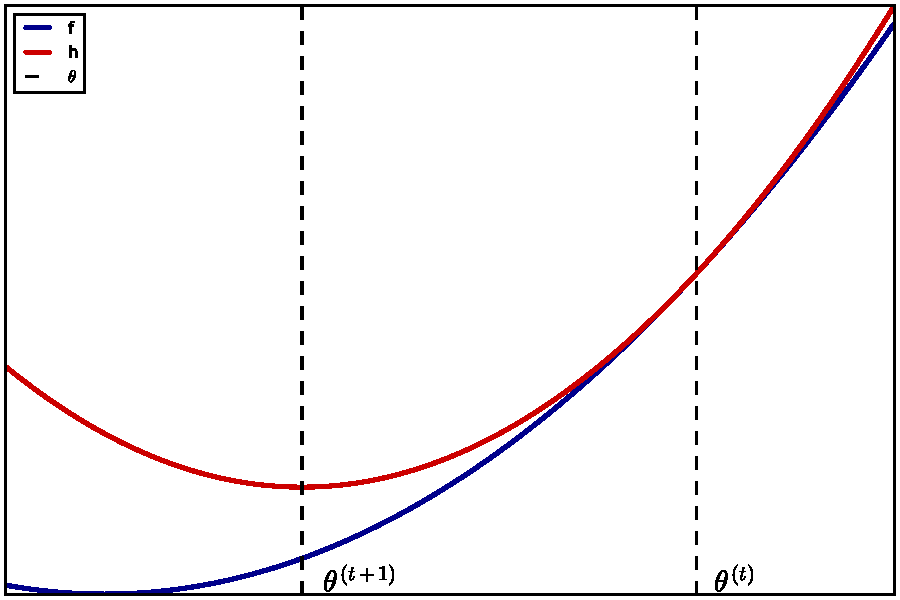
\includegraphics[width=\linewidth]{figures/mmvis.pdf}
  \end{figure}
\end{frame}
\begin{frame}
  \frametitle{What is an Online Algorithm?}
  Velocity can be handled by \emph{online algorithms}
  \begin{itemize}
    \item Input enters piece by piece
    \item Entire dataset is not available at once
    \item A well known example: Stochastic Gradient Descent
    $$\iter{\bm\theta}{t} = \iter{\bm\theta}{t-1} - \gamma_t \nabla f_t(\iter{\bm\theta}{t-1})$$
  \end{itemize}
\end{frame}
\begin{frame}
  \begin{itemize}
    \item The MM principle is common in offline optimization
    \begin{itemize}
      \item Coordinate Descent, Proximal Gradient Method, ADMM, \ldots
    \end{itemize}
    \item Where does it occur in online optimization?
  \end{itemize}
\end{frame}



%%%%%%%%%%%%%%%%%%%%%%%%%%%%%%%%%%%%%%%%%%%%%%%%%%%%%%%%%%%%%%%%%%%%%%%%%%%%%%%%%%%%% SGD as MM
\section{SGD as MM}

%------------------------------------------------ SGD as MM
\subsection{SGD as MM}

\begin{frame}
  \frametitle{Revisit SGD}
  \begin{itemize}
    \item SGD minimizes quadratic approximations of noisy functions
  \end{itemize}
  $$h_t(\bm\theta) = f_t(\iter{\bm\theta}{t-1}) + \nabla f_t(\iter{\bm\theta}{t-1})^T(\bm\theta - \iter{\bm\theta}{t-1}) + \frac{1}{2\gamma_t}\|\bm\theta - \iter{\bm\theta}{t-1}\|_2^2$$
  \vspace{5mm}
  $$\begin{aligned}\iter{\bm\theta}{t} &= \iter{\bm\theta}{t-1} - \gamma_t \nabla f_t(\iter{\bm\theta}{t-1}) \\ &= \argmin_{\bm\theta} h_t(\bm\theta)\end{aligned}$$

\end{frame}
\begin{frame}
  \begin{itemize}
    \item $L$-Lipschitz continuous gradient
    $$f(\bm\theta) \le f(\bm u) + \nabla f(\bm u)^T(\bm\theta - \bm u) + \frac{L}{2}\|\bm\theta - \bm u\|_2^2$$
    \item i.e., there exists a quadratic upper bound
    \item RHS is a majorizing function
  \end{itemize}
\end{frame}
\begin{frame}
  Suppose $f_t(\bm\theta)$ has $L_t$-Lipschitz continuous gradient
  \begin{itemize}
    \item SGD updates are MM updates anytime $\gamma_t^{-1} \le L_t$
  \end{itemize}
\end{frame}
\begin{frame}
  \begin{itemize}
    \item Majorizations get worse over time ($\gamma_t \rightarrow 0$), forcing the parameter to remain near its current state
  \end{itemize}
  \begin{figure}
    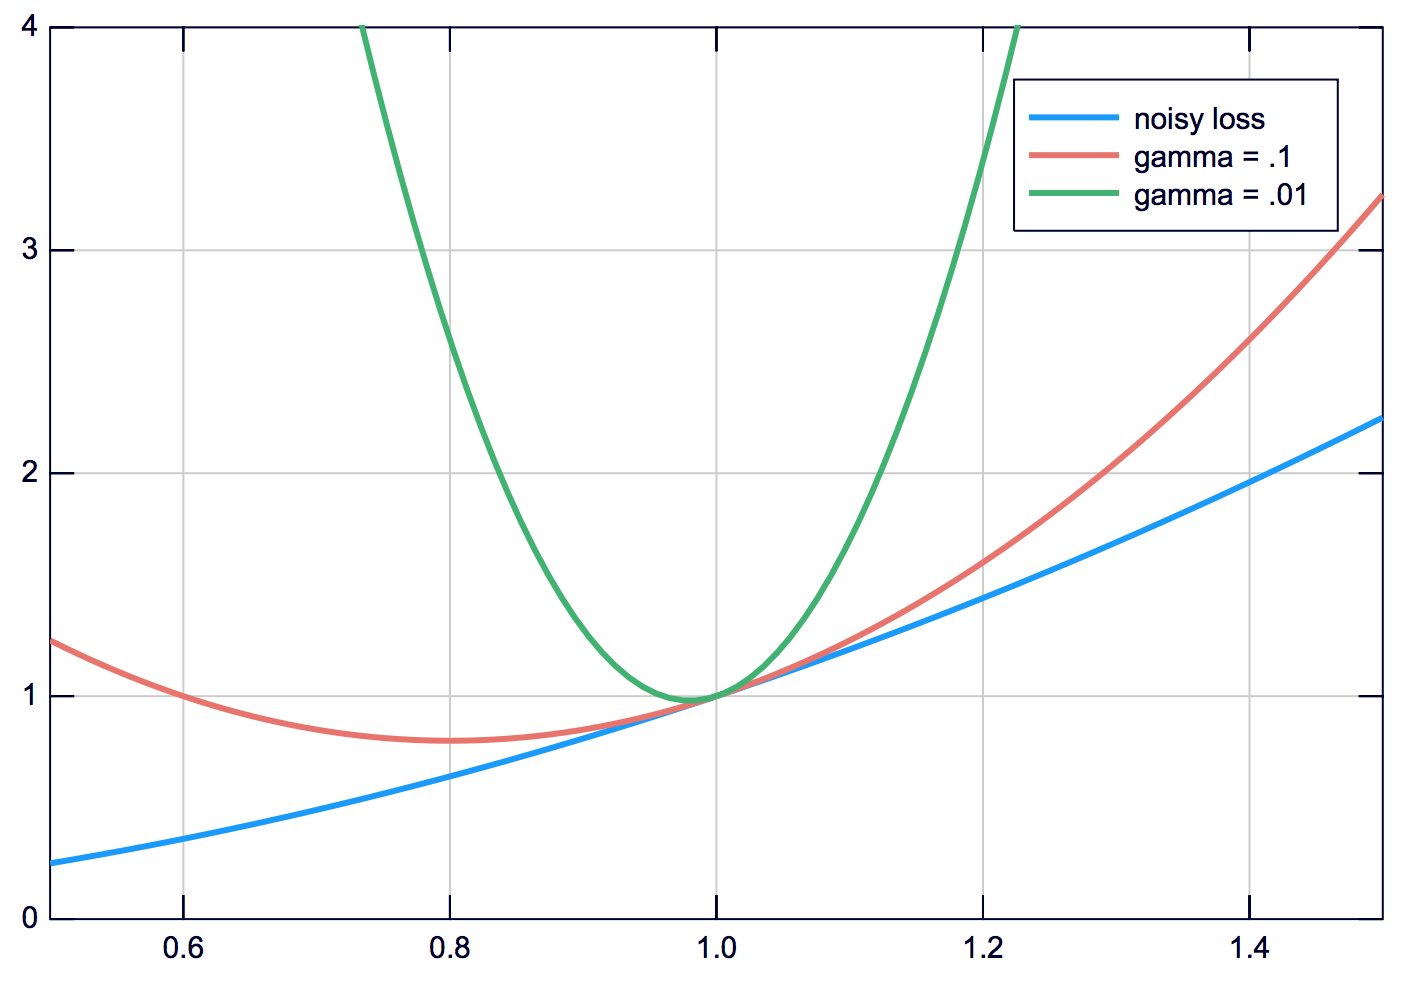
\includegraphics[width=.7\textwidth]{figures/quadraticupperbound.png}
  \end{figure}
\end{frame}



%%%%%%%%%%%%%%%%%%%%%%%%%%%%%%%%%%%%%%%%%%%%%%%%%%%%%%%%%%%%%%%%%%%%%%%%%%%%%%%%%%%%% Online MM
\section{Online MM}
\subsection{Setup}
\begin{frame}
  \frametitle{Online MM}
  \begin{itemize}
    \item Define an Online MM Algorithm as one which follows these steps for each observation/minibatch of data:
  \end{itemize}
  \begin{enumerate}
    \item observe $f_t(\bm\theta)$
    \item create majorization $h_t(\bm\theta)$
    \item Update surrogate objective function $Q_t(\bm\theta)$ with $h_t(\bm\theta)$
    \item $\iter{\bm\theta}{t+1} = argmin_{\bm\theta}Q_t(\bm\theta)$
  \end{enumerate}
\end{frame}
\begin{frame}
  \begin{itemize}
    \item Algorithms differ at steps 2 (the majorization) and 3 (how $Q_t$ is updated)
    \item Ex: SGD
    \begin{itemize}
      \item[-] $h_t=$ quadratic upper bound ($m_t$-strongly convex, $m_t\rightarrow\infty$)
      \item[-] $Q_t(\bm\theta) = h_t(\bm\theta)$
    \end{itemize}
  \end{itemize}
\end{frame}

\subsection{Online MM Types}
\begin{frame}
  \frametitle{Online MM Type 1}
  \begin{itemize}
    \item Rare case when there exists ``sufficient statistics'' for majorizing $\frac{1}{t}\sum_{\tau=1}^t f_\tau(\bm\theta)$ analytically
    \item Online majorization = offline majorization
    \item However, to get same estimate as offline algorithm, we need multiple iterations per update
  \end{itemize}
\end{frame}
\begin{frame}
  \frametitle{Online MM Type 2}
  \begin{itemize}
    \item $Q_t(\bm\theta) = (1 - \gamma_t)Q_{t-1}(\bm\theta) + \gamma_t h_t(\bm\theta)$
    \item Weighted average of surrogate objective and noisy majorization
  \end{itemize}
\end{frame}
\begin{frame}
  \frametitle{Online MM Type 3}
  \begin{itemize}
    \item $Q_t(\bm\theta) = h_t(\bm\theta)$, $h_t$ is $m_t$ strongly convex, $m_t\rightarrow\infty$
    \item SGD-like algorithms (ADAGRAD, ADAM)
    \item Are there non-SGD algorithms?
  \end{itemize}
\end{frame}


\subsection{Translating Offline to Online}
\begin{frame}
  \frametitle{Which types can you use?}
  \begin{figure}
    \begin{itemize}
      \item Type 1? Only if majorization depends on O(1) sufficient statistics
      \item Type 2? Always
      \item Type 3? Only if majorization can get worse as $t\rightarrow\infty$
    \end{itemize}
  \end{figure}
\end{frame}
\begin{frame}
  \frametitle{Can you Make a Majorization "Worse"?}
  \begin{itemize}
    \item[\ding{51}] Quadratic upper bound
      $$h_t(\bm\theta) = f_t(\bm u) + \nabla f_t(\bm u)^T(\bm\theta - \bm u) + \frac{L}{2\gamma_t}\|\bm\theta - \bm u\|_2^2$$
    \item[\ding{55}] Definition of convexity with linear predictor
      $$h_t(\bm x_t^T\bm\beta) = \sum_j \alpha_{tj} f_t\left[\frac{x_{tj}}{\alpha_{tj}}(\beta_j - \iter{\beta_j}{t-1}) + \bm x_t^T\iter{\bm\beta}{t-1}\right]$$
  \end{itemize}
\end{frame}


%%%%%%%%%%%%%%%%%%%%%%%%%%%%%%%%%%%%%%%%%%%%%%%%%%%%%%%%%%%%%%%%%%%%%%%%%%%%%%%%%%%%% MMQD
\section{MMQD}

\subsection{Type 2: MMQD}
\begin{frame}
  Online \textbf{MM} with \textbf{Q}uadratic upper bound using a \textbf{D}iagonal Hessian approximation
\end{frame}
\begin{frame}
  \begin{itemize}
    \item If $\bm H - d^2 f(\bm\theta)$ is nonnegative definite, then
    $$h(\bm\theta) = f(\bm u) + \nabla f(\bm u)^T(\bm\theta - \bm u) + \frac{1}{2}(\bm\theta - \bm u)\bm H(\bm\theta - \bm u)$$
    is a majorizing function
    \item However, parameters only split if $\bm H$ is diagonal
  \end{itemize}
\end{frame}
\begin{frame}
  \begin{itemize}
    \item Online MM with Quadratic Upper Bound is
    $$\iter{\bm\theta}{t} = \bm A_t^{-1}\bm b_t,$$
    where
    $$\begin{aligned}
      \bm A_t &= (1 - \gamma_t)\bm A_{t-1} + \gamma_t \bm H_t \\
      \bm b_t &= (1 - \gamma_t)\bm b_{t-1} + \gamma_t[\bm H_t\iter{\bm\theta}{t-1} - \nabla f_t(\iter{\bm\theta}{t-1})]
      \end{aligned}$$
  \end{itemize}
\end{frame}
\begin{frame}
  \frametitle{Applying regularization}
  For machine learning problems
    $$\frac{1}{n}\sum f_i(\bm\theta) + g(\bm\theta),$$
    the MMQD element-wise updates simplify to
    $$\iter{\theta_j}{t} = \mathbf{prox}_{h_{jj}^{-1}g}\left(\frac{b_{tj}}{h_{jj}}\right)$$
\end{frame}

%%%%%%%%%%%%%%%%%%%%%%%%%%%%%%%%%%%%%%%%%%%%%%%%%%%%%%%%%%%%%%%%%%%%%%%%%%%%%%%%%%%%% Simulations
\section{Simulation}
\subsection{Linear Regression}
\begin{frame}
  \begin{itemize}
    \item The following plots display the average loss of various online algorithms (using several different learning rates) relative to the offline solution for 1000 replications of simulated data.
    \item Solid line: median relative loss
    \item Ribbons: 0.05 and 0.95 quantiles
  \end{itemize}
\end{frame}
\begin{frame}
  \begin{itemize}
    \item Learning Rate: $\gamma_t = t^{-r}, r\in[.5, .7, .9]$
  \end{itemize}
  \begin{figure}
    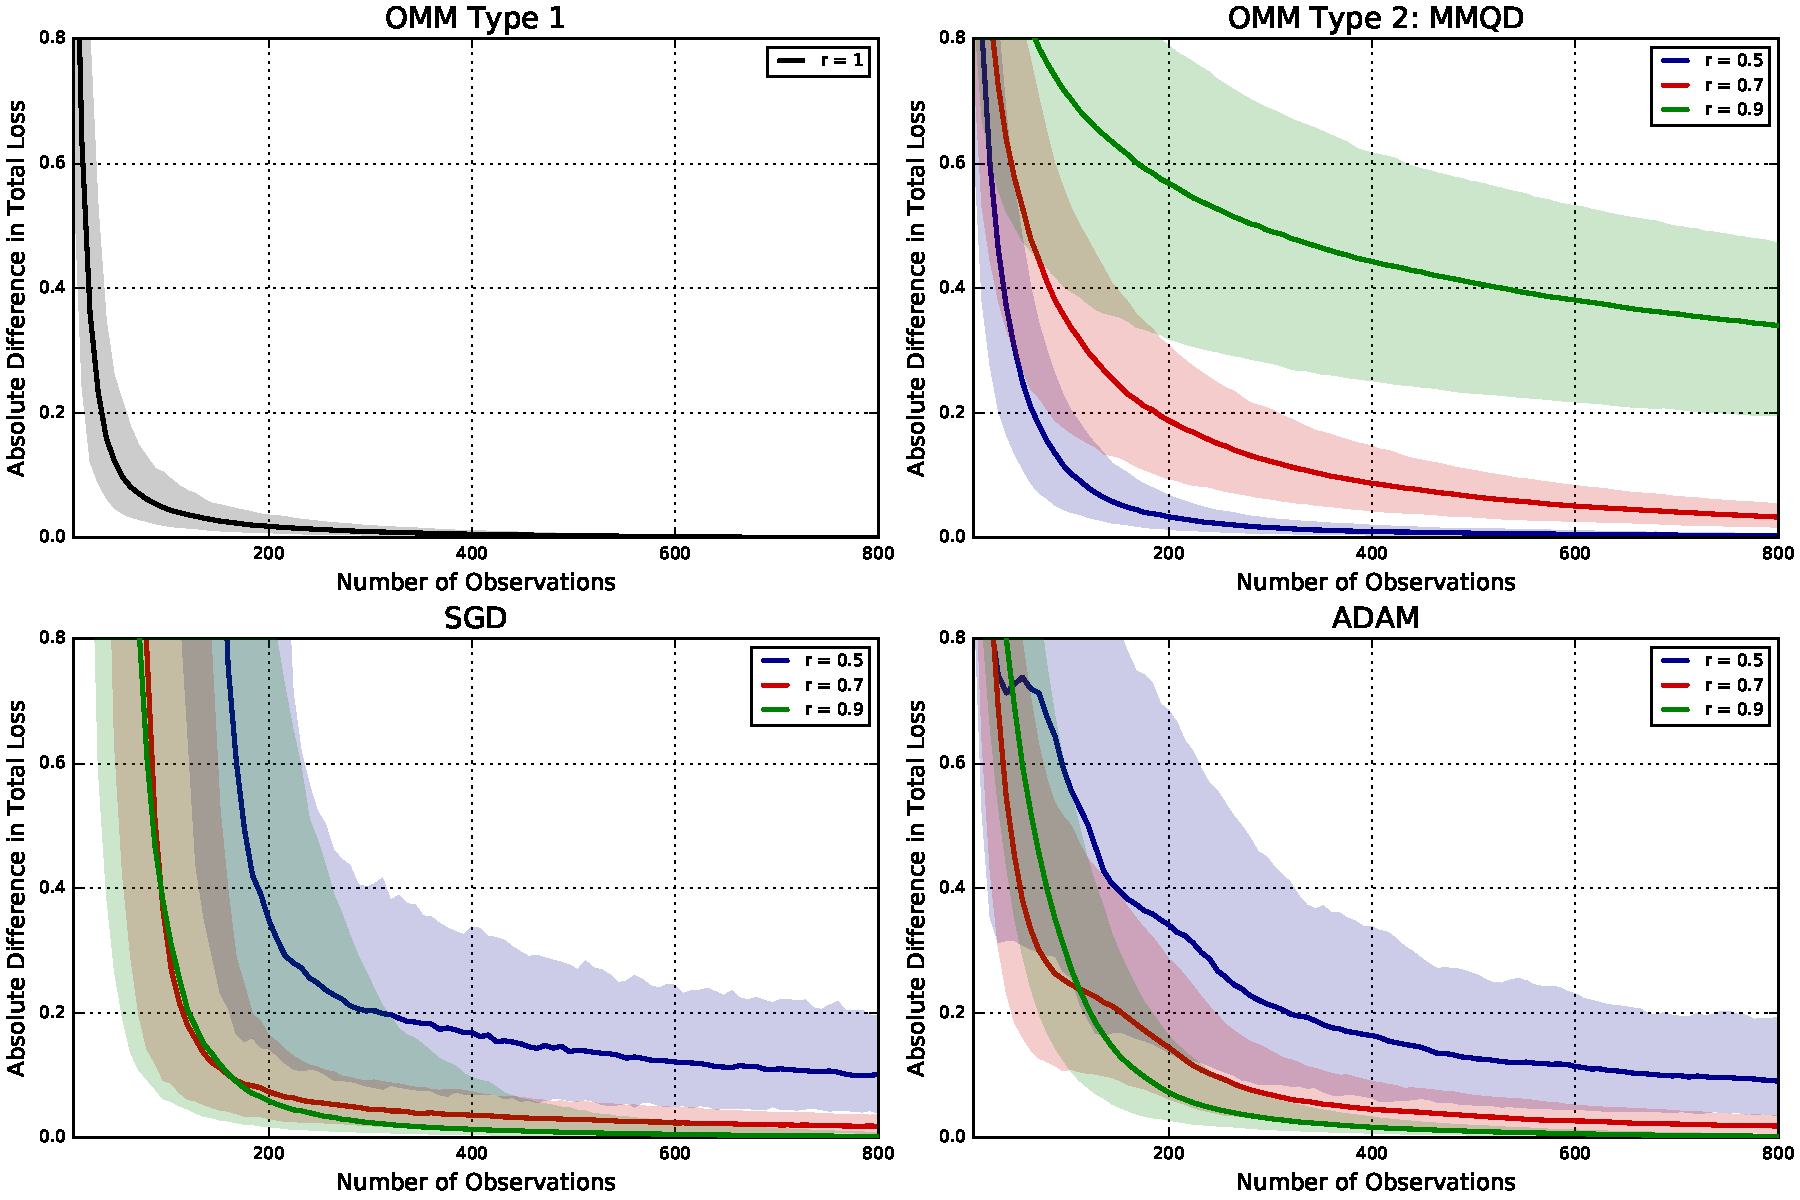
\includegraphics[width=\textwidth]{figures/linregmm_simulation.pdf}
  \end{figure}
\end{frame}

\subsection{Thanks}
\begin{frame}
  \frametitle{Thank You}
  \begin{figure}
    
\includegraphics[width=.2\textwidth]{figures/julia.png}
  \end{figure}
  \begin{itemize}
    \item Software available:
    \begin{itemize}
      \item OnlineStats.jl
      \item OnlineStatsModels.jl
    \end{itemize}
    \item Questions?
  \end{itemize}
\end{frame}




%----------------------------------------------------------------------------------------

\end{document}
